
\section{The Bottleneck Problem}
\begin{frame}{}
  \LARGE \textbf{The Bottleneck Problem}
\end{frame}


\begin{frame}{The Bottleneck Problem}
    \textbf{Fixed-length context vector = information bottleneck}
    \begin{itemize}
        \item[\textcolor{red}{$\blacktriangleright$}] Encoder must \textbf{compress entire input sequence} into a single vector
        \item[\textcolor{red}{$\blacktriangleright$}] Longer or more complex inputs $\rightarrow$ information loss
        \item[\textcolor{red}{$\blacktriangleright$}] Decoder relies solely on that vector to produce outputs
    \end{itemize}
    \vspace{1em}
    \textbf{Leads to poor performance on long sentences or tasks requiring high context awareness}
\end{frame}

\begin{frame}{A problem with this framework} 
  \begin{itemize}
      \item All the information about the input sequence is embedded into a single vector.
      \begin{itemize}
          \item The “hidden” node layer at the end of the input sequence.
          \item This one node is “overloaded” with information, particularly if the input is long.
      \end{itemize}
  \end{itemize}
  \vfill
\end{frame}

\begin{frame}{A problem with this framework}
  \begin{center}
    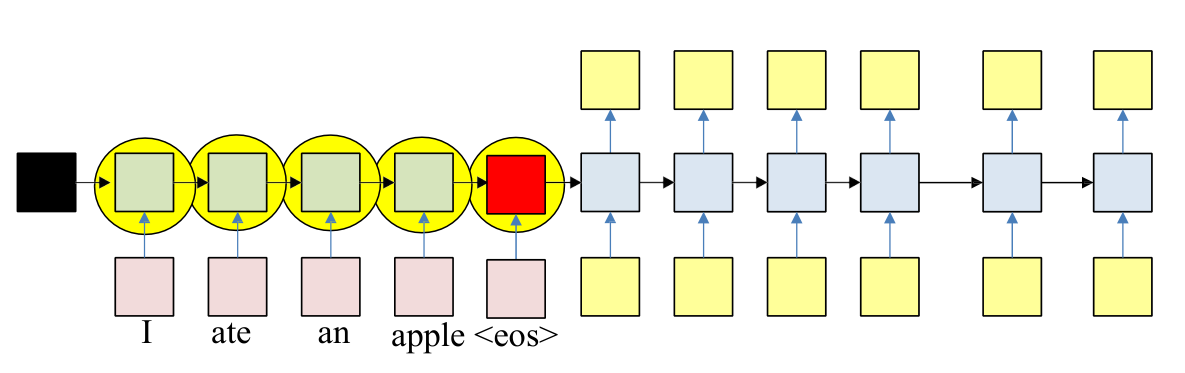
\includegraphics[width=0.35\paperwidth,height=0.35\paperheight,keepaspectratio]{assets/Lecture-4_Sequence_to_Sequence_Models_Intro_to_Attention/slide_024.png}
  \end{center}  
  \begin{itemize}
      \item In reality: All hidden values carry information.
      \begin{itemize}
          \item Some of which may be diluted by the time we get to the final state of the encoder.
      \end{itemize}
  \end{itemize}
  \vfill
\end{frame}

\begin{frame}{A problem with this framework}
  \begin{center}
    
\includegraphics[width=0.35\paperwidth,height=0.35\paperheight,keepaspectratio]{assets/Lecture-4_Sequence_to_Sequence_Models_Intro_to_Attention/slide_025.png}
  \end{center}  
  \begin{itemize}
      \item Every output is related to the input directly.
      \item Not sufficient to have the encoder hidden state to only the initial state of the decoder.
      \item Misses the direct relation of the outputs to the inputs.
  \end{itemize}
  \vfill
\end{frame}

\begin{frame}{}
  \LARGE \textbf{Realization: We Need More Context!}
\end{frame}

\begin{frame}{Realization: We Need More Context!}
  \begin{block}{}
    \textbf{Decoder should have access to all encoder states, not just the final one.}
  \end{block}
  \begin{itemize}
    \item This inspired the development of the \textbf{attention mechanism}.
    \item Instead of passing only the final state, allow the decoder to \textit{``look back''} at \textbf{all input positions}.
  \end{itemize}
\end{frame}

\begin{frame}{Using all input hidden states}
  \begin{center}
    
\includegraphics[width=0.35\paperwidth,height=0.35\paperheight,keepaspectratio]{assets/Lecture-4_Sequence_to_Sequence_Models_Intro_to_Attention/slide_028.png}
  \end{center}  
  \begin{itemize}
      \item Simple solution: Compute the average of all encoder hidden states.
      \item Input this average to every stage of the decoder.
      \item The initial decoder hidden state is now separate from the encoder and may be a learnable parameter.
  \end{itemize}
  \vfill
\end{frame}

\begin{frame}{Using all input hidden states}
  \begin{center}
    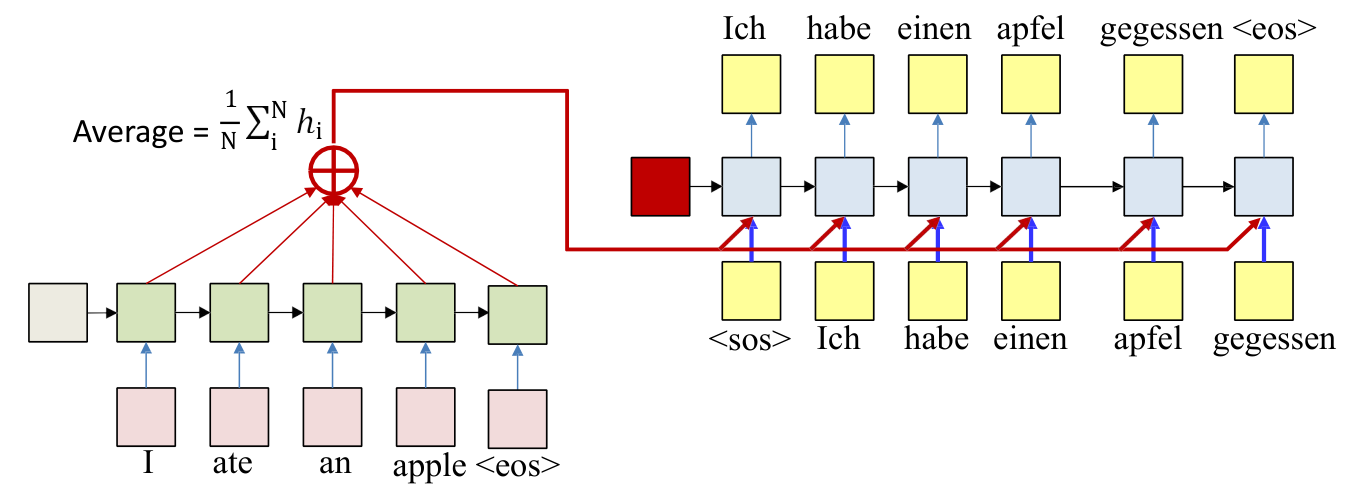
\includegraphics[width=0.35\paperwidth,height=0.35\paperheight,keepaspectratio]{assets/Lecture-4_Sequence_to_Sequence_Models_Intro_to_Attention/slide_029.png}
  \end{center}  
  \begin{itemize}
      \item Problem: The average applies the same weight to every input.
      \item It supplies the same average to every output word.
      \item In practice, different outputs may be related to different inputs.
      \begin{itemize}
          \item E.g., “Ich” is most related to “I”, and “habe” and “gegessen” are both most related to “ate”.
      \end{itemize}
  \end{itemize}
\end{frame}

\begin{frame}{Using all input hidden states}
  \begin{center}
    
\includegraphics[width=0.35\paperwidth,height=0.35\paperheight,keepaspectratio]{assets/Lecture-4_Sequence_to_Sequence_Models_Intro_to_Attention/slide_030.png}
  \end{center}

  \textcolor{red}{\textbf{Solution:} Use a \textit{different} weighted average for each output word}
  \begin{itemize}
    \item The weighted average provided for the $k$th output word is:
    \begin{equation*}
      c_t = \frac{1}{N} \sum_{i} w_i(t) h_i
    \end{equation*}
  \end{itemize}
\end{frame}

\begin{frame}{Using all input hidden states}
\centering
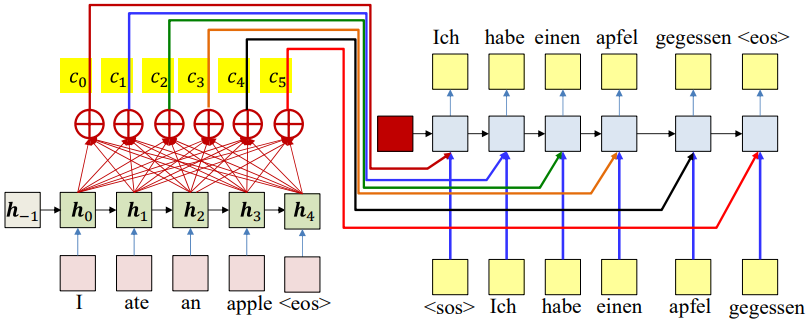
\includegraphics[width=0.35\paperwidth,height=0.35\paperheight,keepaspectratio]{assets/Lecture-4_Sequence_to_Sequence_Models_Intro_to_Attention/slide_031.png}
\begin{equation*}
    c_t = \frac{1}{N} \sum_{i=1}^N w_i(t) h_i
\end{equation*}

\begin{itemize}
    \item This solution will work if the weights $w_{ki}$ can somehow be made to “focus” on the right input word
        \begin{itemize}
            \item E.g., when predicting the word “apfel”, $w_3(4)$, the weight for “apple” must be high while the rest must be low
        \end{itemize}
    \item How do we generate such weights??
\end{itemize}

\end{frame}